\documentclass[11pt,letterpaper]{article}
\PassOptionsToPackage{hyphens}{url}
\usepackage[margin=.83in,top=.8in,bottom=.8in,headheight=15pt]{geometry}
\usepackage[T1]{fontenc}
\usepackage{lmodern,amsmath,amssymb,mathtools,bm,booktabs,array,graphicx,tikz}
\usetikzlibrary{arrows.meta,positioning,calc,decorations.pathreplacing,patterns}
\definecolor{ink}{HTML}{17344D}\definecolor{accent}{HTML}{087E8B}\definecolor{pale}{HTML}{EDF5F5}\definecolor{gold}{HTML}{AD6B19}
\providecommand{\dd}{\,\mathrm{d}}\providecommand{\R}{\mathbb{R}}
\providecommand{\E}{\mathbb{E}}\providecommand{\Var}{\operatorname{Var}}
\providecommand{\Cov}{\operatorname{Cov}}\providecommand{\diag}{\operatorname{diag}}
\providecommand{\norm}[1]{\left\lVert#1\right\rVert}
\providecommand{\abs}[1]{\left|#1\right|}
\usepackage{microtype,hyperref,fancyhdr,enumitem,amsthm,sectsty,needspace}
\allsectionsfont{\raggedright}
\hypersetup{colorlinks=true,linkcolor=ink,urlcolor=accent,pdfauthor={Zan Ahmad},pdftitle={Conservation, viscous flow and transport / CFD notes}}
\setlength{\parindent}{0pt}\setlength{\parskip}{6pt}\linespread{1.07}
\setlist{itemsep=3pt,topsep=4pt,leftmargin=*}
\emergencystretch=2em\clubpenalty=10000\widowpenalty=10000
\pagestyle{fancy}\fancyhf{}\fancyhead[L]{\small Computational Cardiology}\fancyhead[R]{\small Lecture 5--8}
\fancyfoot[L]{\footnotesize Zan Ahmad}\fancyfoot[R]{\footnotesize\thepage}\renewcommand{\headrulewidth}{.3pt}
\newtheorem{proposition}{Proposition}\newtheorem{theorem}{Theorem}\newtheorem{lemma}{Lemma}
\theoremstyle{definition}\newtheorem{definition}{Definition}\newtheorem{example}{Example}
\numberwithin{equation}{section}
\begin{document}
{\small\scshape Computational Cardiology\hfill Lecture 5--8}\par\medskip
{\raggedright\hyphenpenalty=10000\exhyphenpenalty=10000\LARGE\bfseries\color{ink} Conservation, viscous flow and transport\par}\medskip
{\small CFD notes}\par\bigskip

\noindent\href{../../m05/slides.html}{Lecture 5: fluxes}\quad
\href{../../m06/slides.html}{Lecture 6: error}\quad
\href{../../m07/slides.html}{Lecture 7: momentum}\quad
\href{../../m08/slides.html}{Lecture 8: geometry}\quad
\href{index.html}{Examples and animation}

\Needspace{10\baselineskip}\section{A flow field and a conservation law}
Let $\Omega\subset\mathbb R^3$ denote a fixed fluid region. The velocity $\boldsymbol u(\boldsymbol x,t)$ has units of length per time, whereas the pressure $p(\boldsymbol x,t)$ has units of force per area. A velocity vector tells us where a fluid particle moves. A pressure gradient contributes to its acceleration. The two quantities cannot be interchanged, even when arrows and colors are used to display both.

For a fixed control volume $K$ with outward normal $\boldsymbol n$, mass conservation is
\begin{equation}\frac{\mathrm d}{\mathrm dt}\int_K\rho\,\mathrm dV
=-\int_{\partial K}\rho\boldsymbol u\cdot\boldsymbol n\,\mathrm dS.\end{equation}
Assume constant density $\rho>0$. Since the relation holds for every suitable $K$, the divergence theorem gives $\nabla\cdot\boldsymbol u=0$. This constrains the local expansion of the velocity field. It does not say that speed is constant or that the fluid cannot accelerate.

For a passive concentration $c$ and constant diffusivity $D\ge0$, define the flux
\begin{equation}\boldsymbol j=c\boldsymbol u-D\nabla c.\end{equation}
With no internal source, the corresponding budget is
\begin{equation}\frac{\mathrm d}{\mathrm dt}\int_K c\,\mathrm dV
=-\int_{\partial K}\boldsymbol j\cdot\boldsymbol n\,\mathrm dS,
\qquad \partial_t c+\nabla\cdot(c\boldsymbol u)=D\Delta c.\end{equation}
Here $D$ has units $\mathrm{m^2/s}$. Advective and diffusive fluxes have the same dimensions. If $c$ is divided by a reference concentration, the stored quantity per unit out-of-plane width in two dimensions has units of area.

\Needspace{10\baselineskip}\section{Momentum and the pressure constraint}
For an incompressible Newtonian fluid of constant viscosity $\mu$, balance of momentum gives
\begin{equation}\rho\left(\partial_t\boldsymbol u+(\boldsymbol u\cdot\nabla)\boldsymbol u\right)
=-\nabla p+\mu\Delta\boldsymbol u+\boldsymbol f,
\qquad \nabla\cdot\boldsymbol u=0.\end{equation}
The material acceleration includes both local time variation and motion through a spatially varying field. The viscous term arises from the stress $2\mu\boldsymbol D(\boldsymbol u)$, where
$\boldsymbol D(\boldsymbol u)=(\nabla\boldsymbol u+\nabla\boldsymbol u^{T})/2$.
The incompressible pressure enforces a constraint; it is not obtained from a compressible equation of state in this model. Adding a spatially constant value to pressure leaves the velocity equation unchanged. A pressure reference is therefore needed when the boundary data do not otherwise fix it.

Choose scales $L,U$ and $L/U$ for length, speed and time. Scaling pressure by $\rho U^2$ gives the dimensionless viscous coefficient $1/\mathrm{Re}$, where
\[\mathrm{Re}=\frac{\rho UL}{\mu}.\]
A small Reynolds number motivates neglecting inertia only after the relevant geometry, scales and unsteadiness have been considered. A low value is not a numerical stability condition.

\Needspace{10\baselineskip}\section{Initial and boundary data are part of the model}
A transient velocity requires initial data consistent with incompressibility and the imposed boundary conditions. On a fixed impermeable no-slip wall, $\boldsymbol u=0$. On a moving no-slip wall, the fluid velocity equals the wall velocity. At an inlet, a prescribed profile fixes the incoming volume flux; an outlet might prescribe traction, pressure under a suitable formulation, or coupling to a reduced downstream model. Arbitrarily prescribing both pressure and all velocity components on the same boundary generally overdetermines the problem.

The scalar problem has its own boundary data. An inlet concentration specifies material entering the region. At an impermeable wall, $\boldsymbol j\cdot\boldsymbol n=0$. A zero diffusive outlet flux, $\nabla c\cdot\boldsymbol n=0$, still permits advective material to leave. It is not a zero-total-flux condition. The direction of the flow matters when using inflow/outflow conditions.

\Needspace{10\baselineskip}\section{A fully developed channel calculation}
Consider stationary walls at $y=0,H$ and a velocity $\boldsymbol u=(u(y),0,0)$. Let $-\partial_xp=G\ge0$ and take no body force. Steady fully developed motion has zero convective acceleration, so the momentum equation reduces exactly to
\begin{equation}\mu u''=-G,\qquad u(0)=u(H)=0.\end{equation}
Integrating twice and applying the boundary values yields
\begin{equation}u(y)=\frac{G}{2\mu}y(H-y),\quad
u_{\max}=\frac{GH^2}{8\mu},\quad
q=\int_0^H u(y)\,\mathrm dy=\frac{GH^3}{12\mu}.\end{equation}
In this display $u_{\max}$ denotes the maximum speed; $q$ is volume flux per width, in $\mathrm{m^2/s}$. The total volume flux through width $W$ is $Q=Wq$.

For $H=2\,\mathrm{mm}$, $G=100\,\mathrm{Pa/m}$ and $\mu=0.004\,\mathrm{Pa\,s}$, the maximum speed is $12.5\,\mathrm{mm/s}$ and the mean speed is $8.333\ldots\,\mathrm{mm/s}$. Over $L=20\,\mathrm{mm}$ the pressure drop is $GL=2\,\mathrm{Pa}$. Choosing $W=10\,\mathrm{mm}$ gives $Q=0.1667\,\mathrm{mL/s}$. This is a planar benchmark; the cubic dependence on gap must not be confused with the fourth-power radius dependence for a circular pipe.

\begin{center}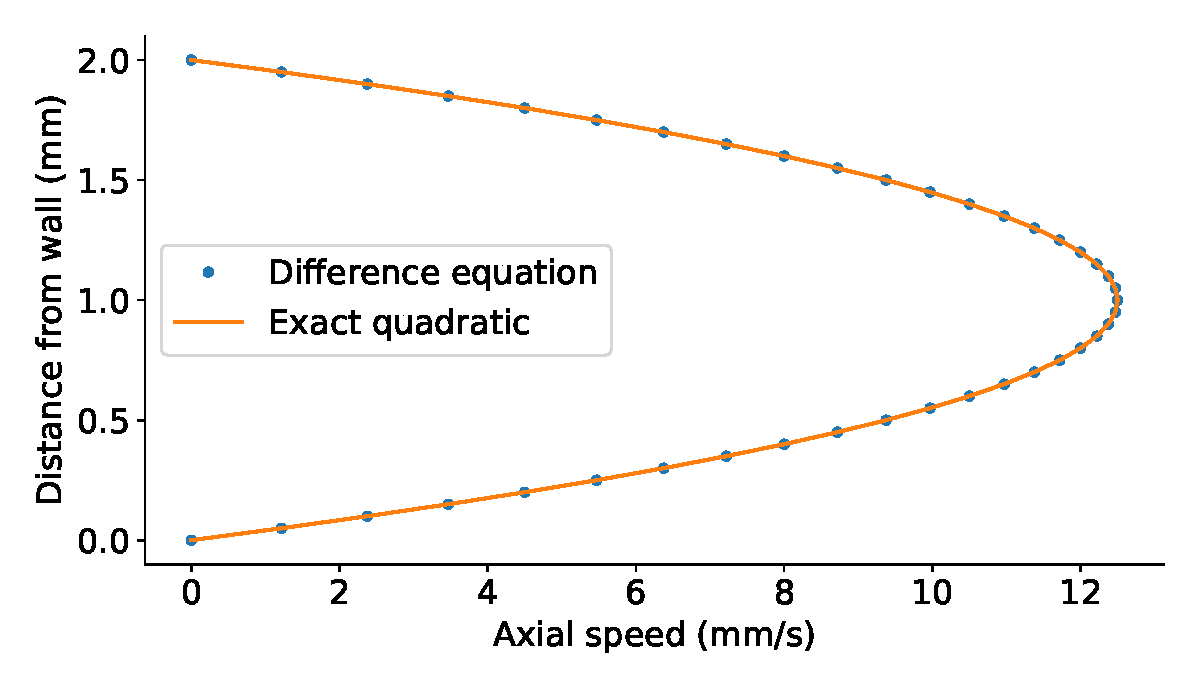
\includegraphics[width=.8\linewidth]{results/velocity.pdf}\end{center}

\Needspace{10\baselineskip}\section{From the differential equation to a linear system}
On $y_i=ih$, $h=H/N$, approximate the second derivative by
\[\frac{u_{i-1}-2u_i+u_{i+1}}{h^2}=-\frac G\mu,\qquad i=1,\ldots,N-1.\]
The resulting tridiagonal system has diagonal entries $2$, off-diagonals $-1$ and right-hand side $Gh^2/\mu$, with boundary values moved to the right-hand side. For homogeneous walls it is positive definite: extend a vector by $z_0=z_N=0$ and compute
\[z^TAz=\sum_{i=0}^{N-1}(z_{i+1}-z_i)^2>0\quad\text{when }z\ne0.\]
The quadratic exact solution also satisfies this difference equation exactly at the nodes, up to roundoff. Consequently this particular profile cannot reveal the generic truncation order. Trapezoidal integration of the same samples still has a relative flux error $1/N^2$. A small algebraic residual, a small discretization error and accurate postprocessing are three different statements.

A general incompressible solver has coupled velocity/pressure unknowns, for example a block system with momentum, gradient and divergence blocks. Pressure correction and coupled saddle-point approaches are ways of enforcing both equations. Our code solves only the reduced channel boundary-value problem, then uses its analytic velocity in the transport experiment. It does not implement a general three-dimensional Navier--Stokes solver.

\Needspace{10\baselineskip}\section{A conservative two-dimensional transport experiment}
Use the rectangle $[0,L]\times[0,H]$, initially with $c=0$. Apply $c_{\rm in}=1$ for $0\le t<0.3\,\mathrm s$ and zero afterward. Take $D=2\times10^{-6}\,\mathrm{m^2/s}$ as a chosen teaching parameter. It is not a fitted blood diffusivity. Walls have zero normal scalar flux; the outlet has zero diffusive flux.

For cell averages $c_{ij}$ with spacings $\Delta x,\Delta y$, write
\begin{equation}c_{ij}^{n+1}=c_{ij}^n-\Delta t\left[
\frac{F_{i+1/2,j}-F_{i-1/2,j}}{\Delta x}+
\frac{G_{i,j+1/2}-G_{i,j-1/2}}{\Delta y}\right].\end{equation}
Because $u_j\ge0$, an interior axial face uses the upwind advective flux and centered diffusive flux,
\[F_{i+1/2,j}=u_jc_{ij}-D\frac{c_{i+1,j}-c_{ij}}{\Delta x},\qquad
G_{i,j+1/2}=-D\frac{c_{i,j+1}-c_{ij}}{\Delta y}.\]
The inlet boundary is half a cell width from its first center, so its diffusive contribution is $-2D(c_{0j}-c_{\rm in})/\Delta x$. The outlet face uses $u_jc_{N_x-1,j}$. Every interior face flux is computed once and used with opposite signs by its two neighboring cells.

A sufficient nonnegative-coefficient condition for this implementation is
\[\Delta t\left(\frac{\max_j u_j}{\Delta x}
+\frac{3D}{\Delta x^2}+\frac{2D}{\Delta y^2}\right)\le1.\]
The factor $3$ covers the first cell's inlet half-width diffusion plus its interior face. This is a sufficient bound for the stated stencil and boundary treatment, not a universal CFD rule. The implementation uses a factor $0.9$, aligns time steps with the pulse cutoff and applies no clipping.

\begin{center}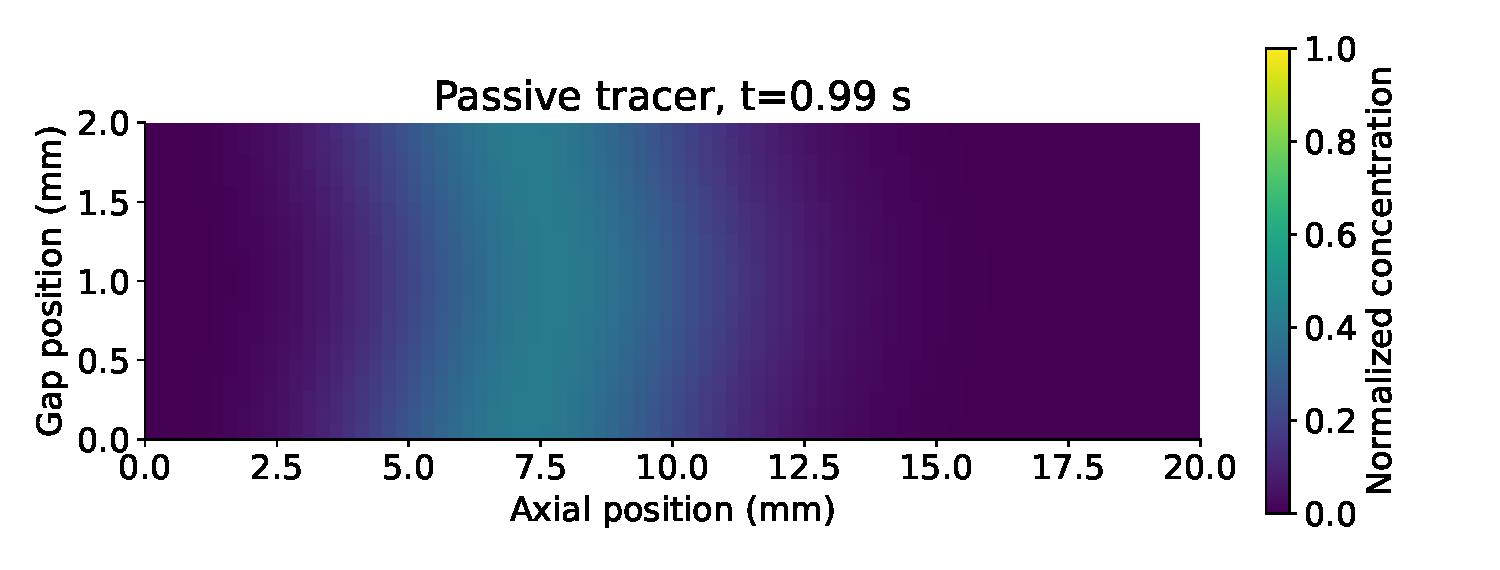
\includegraphics[width=.98\linewidth]{results/tracer-1.pdf}\end{center}
The center of the packet is carried faster than material near the no-slip walls. Diffusion spreads concentration across the shear. A picture alone cannot distinguish physical spreading from upwind numerical diffusion; vary $D$ and the mesh separately.

\Needspace{10\baselineskip}\section{Verification and interpretation}
Let $M^n=\sum_{ij}c_{ij}^n\Delta x\Delta y$. Summing the update cancels all shared interior fluxes, leaving
\[M^{n+1}-M^n=\Delta t\,\Delta y\sum_j
(F_{-1/2,j}-F_{N_x-1/2,j}).\]
The supplied run checks this identity at every step. It also checks the quadratic velocity, linear response to $G$, zero forcing, the constant concentration state, the $D=0$ limit and nonnegative concentrations. The baseline maximum budget defect is about $2.4\times10^{-20}\,\mathrm{m^2}$. That checks the discrete budget, not anatomical or clinical validity.

\begin{center}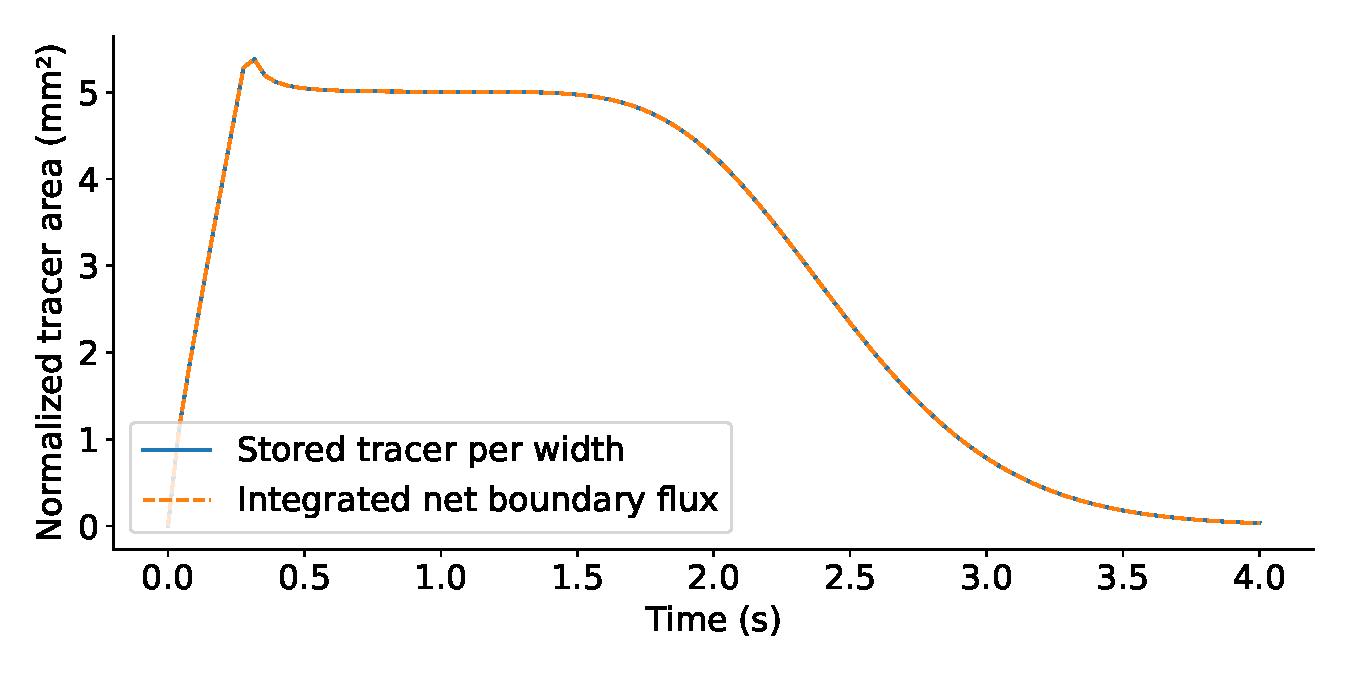
\includegraphics[width=.87\linewidth]{results/budget.pdf}\end{center}
Mesh sensitivity is assessed on the same geometry, pulse and final physical time. At $t=1\,\mathrm s$, stored tracer per width on meshes $(20,8)$, $(40,16)$ and $(80,32)$ is approximately $5.0446$, $5.0121$ and $5.0034$ times $10^{-6}\,\mathrm{m^2}$. This short comparison is evidence of sensitivity; it does not establish a universal convergence order or validation against a measured flow.

A bulk turnover scale $V/Q$ is useful dimensionally but is not the residence time of every particle. Near-wall slow motion, recirculation and unsteady flow can create a broad distribution of transit times. The channel packet demonstrates nonuniform transport even without recirculation. A clinical stasis claim would require a defined quantity, an appropriate model, uncertainty analysis and relevant observations.

\Needspace{10\baselineskip}\section{Experiments and exercises}
\begin{enumerate}
\item Reproduce the baseline with \texttt{python channel\_transport.py --output results}. Identify the columns of \texttt{mass-budget.csv} and explain the sign of net boundary inflow after the inlet pulse has stopped.
\item Double $G$. Predict the change in $u_{\max}$, $q$ and $L/\bar u$ before running the model. Does the entire concentration field simply double? Explain why.
\item Repeat the tracer experiment with $D=0$ and with half the baseline $D$. Refine the mesh separately. Identify a visual change attributable to transport discretization rather than a changed physical parameter.
\item Derive the telescoping mass balance. Explain why replacing a cell average by a clipped value after an unstable step would generally destroy it.
\item Derive the velocity and flux when the upper wall moves at speed $U_w$. Identify which superposition argument permits the calculation.
\item A simulation conserves mass and has a small solver residual. Give two remaining numerical checks and two kinds of information needed before a patient-specific interpretation would be warranted.
\end{enumerate}

\section*{Connections and readings}
\href{../../m05/notes.pdf}{Lecture 5 notes} develop one-dimensional finite volumes; \href{../../m06/notes.pdf}{Lecture 6} separates Fourier-mode space and time errors; \href{../../m07/notes.pdf}{Lecture 7} treats the boundary-value solve; \href{../../m08/notes.pdf}{Lecture 8} distinguishes prescribed kinematics from a momentum solution. \href{channel_transport.py}{The source code} and \href{results/verification.json}{numerical checks} accompany this module.

Hoppensteadt and Peskin, \emph{Modeling and Simulation in Medicine and the Life Sciences}, second edition, develops the conservation-based modeling viewpoint. Ahmad et al., \emph{Optimal Fenestration of the Fontan Circulation} (2022), DOI \href{https://doi.org/10.3389/fphys.2022.867995}{10.3389/fphys.2022.867995}, couples compartmental hemodynamics and oxygen transport. That reduced circulatory model is distinct from the spatial channel calculation here. The existing circulation feedback project remains a separate course project.
\end{document}
